%%% LaTeX Template: Article/Thesis/etc. with colored headings and special fonts
%%%
%%% Source: http://www.howtotex.com/
%%% Feel free to distribute this template, but please keep to referal to http://www.howtotex.com/ here.
%%% February 2011
%%%
%%% Modified January 2016 by CDM

%%%  Preamble
\documentclass[11pt,letterpaper]{article}
\usepackage[margin=1.0in]{geometry}
\usepackage[T1]{fontenc}
\usepackage[bitstream-charter]{mathdesign}
\usepackage[latin1]{inputenc}					
\usepackage{amsmath}						
\usepackage{xcolor}
\usepackage{cite}
\usepackage{hyphenat}
\usepackage{graphicx}
\usepackage{float}
\usepackage{subfigure}
\usepackage{sectsty}
\usepackage[compact]{titlesec} 
\usepackage[tablegrid]{vhistory}
\usepackage{pbox}
\allsectionsfont{\color{accentcolor}\scshape\selectfont}

%%% Definitions
\definecolor{accentcolor}{rgb}{0.0,0.0,0.5} 
\newcommand{\teamname}{Team Epsilon}
\newcommand{\productname}{SCARA Robot Arm}
\newcommand{\coursename}{CSE 4317: Senior Design II}
\newcommand{\semester}{Fall 2016}
\newcommand{\docname}{Architectural Design Specification}
\newcommand{\department}{Department of Computer Science \& Engineering}
\newcommand{\university}{The University of Texas at Arlington}
\newcommand{\authors}{Thomas Zachry \\ Diane Chin \\ Shayan Raza \\ Charlie Pan \\ Randy Thien Chao}

%%% Headers and footers
\usepackage{fancyhdr}
	\pagestyle{fancy}						% Enabling the custom headers/footers
\usepackage{lastpage}	
	% Header (empty)
	\lhead{}
	\chead{}
	\rhead{}
	% Footer
	\lfoot{\footnotesize \teamname \ - \semester}
	\cfoot{}
	\rfoot{\footnotesize page \thepage\ of \pageref{LastPage}}	% "Page 1 of 2"
	\renewcommand{\headrulewidth}{0.0pt}
	\renewcommand{\footrulewidth}{0.4pt}

%%% Change the abstract environment
\usepackage[runin]{abstract}			% runin option for a run-in title
%\setlength\absleftindent{30pt}			% left margin
%\setlength\absrightindent{30pt}		% right margin
\abslabeldelim{\quad}	
\setlength{\abstitleskip}{-10pt}
\renewcommand{\abstractname}{}
\renewcommand{\abstracttextfont}{\color{accentcolor} \small \slshape}	% slanted text

%%% Start of the document
\begin{document}

%%% Cover sheet
{\centering \huge \color{accentcolor} \sc \textbf{\department \\ \university} \par}
\vspace{1 in}
{\centering \huge \color{accentcolor} \sc \textbf{\docname \\ \coursename \\ \semester} \par}
\vspace{0.5 in}
\begin{figure}[h!]
	\centering
   	
\includegraphics[width=0.60\textwidth]{images/final_team_logo_edit}
\end{figure}
\vspace{0.5 in}
{\centering \huge \color{accentcolor} \sc \textbf{\teamname \\ \productname} \par}
\vspace{0.5 in}
{\centering \large \sc \textbf{\authors} \par}
\newpage


%\vspace{1 in}
%\centerline{January 13th, 2012}
%\newpage

%%% Revision History
\begin{versionhistory}
  	\vhEntry{0.1}{11.15.2016}{DC}{document creation}
  	\vhEntry{0.2}{11.30.2016}{DC}{complete first draft}
  	\vhEntry{0.3}{12.02.2016}{DC}{finalized tables}
  	\vhEntry{1.0}{12.07.2016}{DC}{final draft release}
  	\vhEntry{1.1}{12.09.2016}{DC}{added final revisions}
\end{versionhistory}
\newpage

%%% Table of contents
\setcounter{tocdepth}{2}
\tableofcontents
\newpage

%%% List of figures and tables (optional)
\listoffigures
\listoftables
\newpage

%%% Document sections
\section{Introduction}


Your introduction should describe your product concept in sufficient detail that the architectural design will be easy to follow. The introduction may include information used in the first sections of your SRS for this purpose. At a minimum, ensure that the product concept, scope and key requirements are described.

\subsection{Product Concept}
This section describes the purpose, use and intended user audience for the SCARA Robot Arm product.
The SCARA Robot Arm is a system that performs typical industrial sorting routines. Users of the SCARA
Robot Arm will be able to use the SCARA Robot Arm to efficiently sort various common industrial objects. Through the use of a GUI, the user will also be able to control the arm and view both the camera feed and simulation. This way the user is able to have a product that can automate tasks such as sorting as well as be able to configure and control how it accomplishes such tasks.

\subsection{Product Scope}

The SCARA Robot Arm consists of the skeleton of the arm, two motors for joint movement, two encoders, a linear actuator that moves the end effector to grip objects, and an air pump. This hardware receives movement commands from the teensy board and the C code on that, which receives data from an ubuntu OS. The GUI and OpenRave are run on ubuntu, with OpenRave handling the kinematics and movement plans for the robot arm and recieving data from the camera to make its plans. The GUI takes this data and shows it on the screen as well as is responsible for sending the data into packets to the teensy board. 



\subsection{Key Requirements}
 
\setlength{\arrayrulewidth}{1mm}
\setlength{\tabcolsep}{18pt}
\renewcommand{\arraystretch}{2.5}

 
\begin{tabular}{ |p{1cm}|p{5cm}|p{7cm}|  }


\hline
No.& Name &Description \\
\hline
1 & The system shall have the operational design of a SCARA Robot Arm &The design will have the design properties of a SCARA Robot Arm. The Arm will have multiple pivoting joints to aid in movement.  \\
2 & The system shall have a operating area of no more than 18 inches by 18 inches.    & The operating area of the SCARA Robot ARM will have a operation area of minimum 18 inches by 18 inches.  \\
3 &The system shall be a stand alone SCARA Robot Arm with no desktop computer terminal connections for support. & The Robot arm will be designed with no outside user terminal support connections. The arm will have a built in user interface.  \\
4    &The system shall have a minimum of 2 segment links for articulation.  & The Robot Arm will have at least 2 articulating segments in the arm \\
5 & The system shall utilize available technology for computer vision processes & The Arm will use current available technologies for computer vision processes, i.e. cameras, i.r. sensors, high frequency sound emmiters, laser imagers.  \\
6 & The system shall perform current industry accepted sorting processes. & The Robot Arm will perform processes that are currently being utilised in industry, i.e. sorting, object recognition, pick and place.   \\
7 & The system shall incorporate current object recognition technologies. & The Robot Arm will use the current methods to perform object recognition in accordance with processes, i.e. openCV, simpleCV \\
8 & The system shall be contained in 1 compact operational package. & The Robot Arm's final structural form will be one complete working package containing all components needed of the Arm.  \\
9 & The system shall contain sufficient power supply to feed all components of the SCARA Robot Arm. & The Robot Arm and all its dependent components will be supplied power through on board power supplies within the compact package. \\

\hline
\end{tabular}

\setlength{\arrayrulewidth}{1mm}
\setlength{\tabcolsep}{18pt}
\renewcommand{\arraystretch}{2.5}
 
\begin{tabular}{ |p{1cm}|p{5cm}|p{7cm}|  }

\hline
No.& Name &Description \\
\hline

10 & The system shall have a repeatability accuracy of minimum .050mm. & The SCARA Robot Arm will have accuracy to repeatedly focus the end effector within a range of .05mm. \\
11 & The system shall have a resolution accuracy of +- 1mm. & The Robot Arm will have a calculating system to acquire objects within 1mm of its actual position. \\
12 & The system shall adhere to all industry standards for machine power/ lockout safety.  & The SCARA Robot Arm will adhere to all OSHA 3102 standards covering all power supplying power to machinery and all power lockout processes. \\
13 & The system shall follow all OSHA guidelines for robotic machines.  & The SCARA Robot Arm will conform to all OSHA 29 CFR 1910 guidelines for robotic equipment. \\
14 & The system shall allow access for mandatory use period servicing.  & The Robot Arm will allow for the ability to have regular interval maintenence performed.  \\
15 & The system shall contain interface for technician calibration.  & AGO \\
16 & The system shall contain method for system updates delivered through compact disk/usb flash drive. & The Robot Arm shall have the ability for software and firmware updates through either compact disk or through usb flash drive.  \\
\hline

\end{tabular}

\newpage
\section{System Overview}
Lorem ipsum dolor sit amet, quidam omnesque ea vis. Eum an aliquip legendos recusabo. Mea ex purto natum, ne movet fuisset sit. Labore audiam eos ad, facer ornatus posidonium ne ius, et eos duis delenit nusquam.
\newpage
\section{Data Flow}
This section illustrates how the various subsystems interact within the SCARA robot arm. Each flow of data is
identified with an arrow to the direction of the subsystem it sends data towards, as well as indicates what sort of data is being transfered. The subsections provide a high level
overview of the system and the data flows between each of the layers and subsystems as well as
describe how individual data elements are used. 

\begin{figure}[h!]
	\centering
 	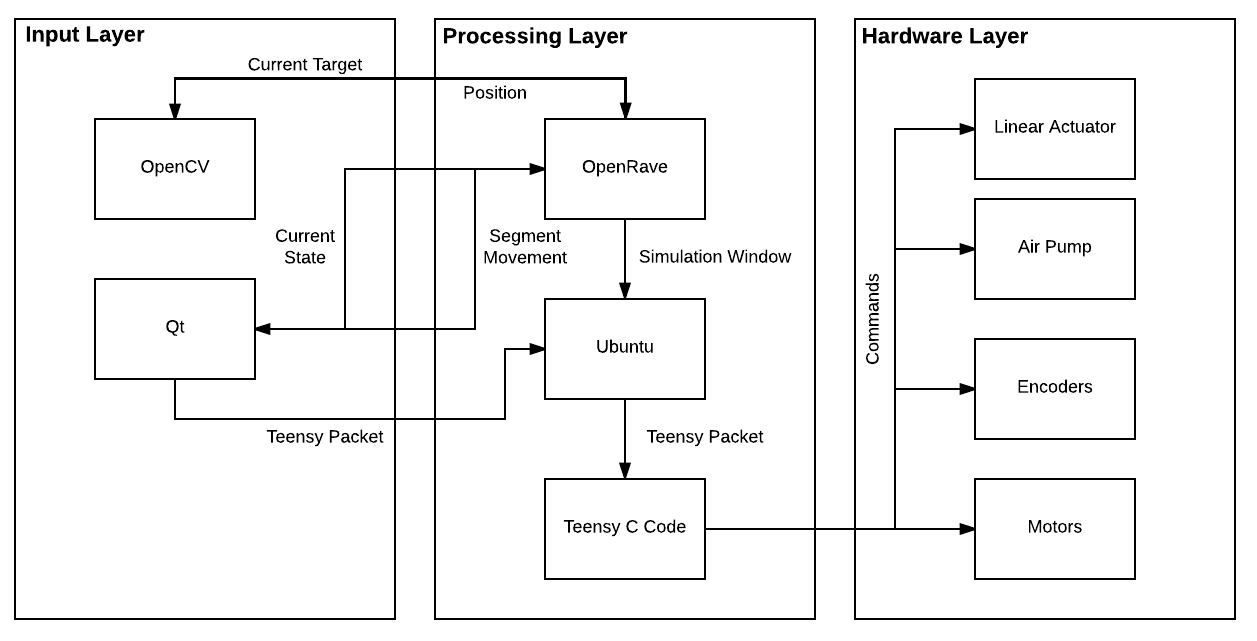
\includegraphics[width=\textwidth]{images/ADS_dataflow}
 \caption{A data flow diagram of the arm}
\end{figure}

\subsection{Data Flow Diagram}
The data flow diagram consists of three layers. Data starts at the Input Layer which is inputted through but the GUI application and the camera with OpenCV. The input layer then sends to the Processing
Layer which is responsible handling and calculating the input data. Then, the processing layer will send its commands to the Hardware layer, which will then execute these commands physically as output.
\newpage
\section{Input Layer Subsystems}
In this section, the layer is described in some detail in terms of its specific subsystems. Describe each of the layers and its subsystems in a separate chapter/major subsection of this document. The content of each subsystem description should be similar. Include in this section any special considerations and/or trade-offs considered for the approach you have chosen.

\begin{figure}[h!]
	\centering
 	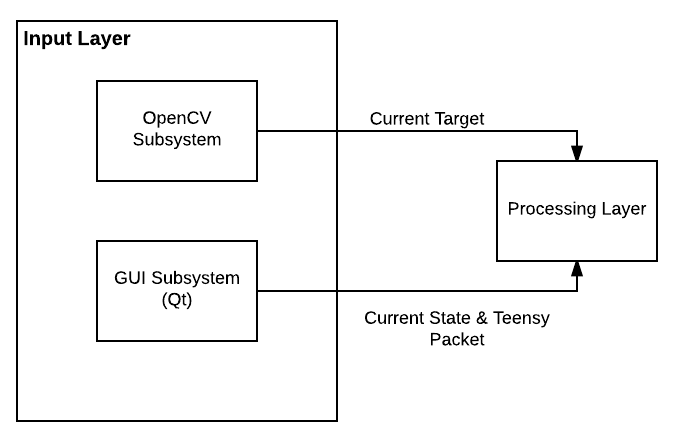
\includegraphics[width=0.60\textwidth]{images/input}
 \caption{Input Layer subsystem diagram}
\end{figure}

\subsection{GUI Subsystem (Qt)}
The purpose of the GUI subsystem is to provide an interface for the user to operate and control the system, as well as see its processes.

\subsubsection{Assumptions}
The GUI should be able to show the camera feed as well as the OpenRave simulation on the screen, and should be able to receive and send this information

\subsubsection{Responsibilities}
The GUI subsystem will be responsible for rendering and displaying the user interface, along with the live camera feed and the Openrave simulation. This UI will also generate events to the system when the user interacts with anything interactible on the interface.

\subsubsection{Subsystem Interfaces}


\begin {table}[H]
\caption {GUI interfaces} 
\begin{center}
    \begin{tabular}{ | p{1cm} | p{6cm} | p{3cm} | p{3cm} |}
    \hline
    ID & Description & Inputs & Outputs \\ \hline
    \#1 & Data gets stored as a data packet to send to the Processing Layer & \pbox{3cm}{Event generated by the application} & \pbox{3cm}{None}  \\ \hline

    \end{tabular}
\end{center}
\end{table}

\subsection{OpenCV Subsystem}
The OpenCV Subsystem is what is able to take and show the camera feed.

\subsubsection{Assumptions}
The OpenCV subsystem will be able to take the camera feed and be able to determine the current target to give to the processing layer.

\subsubsection{Responsibilities}
The OpenCV subsystem will be responsible for processing the camera feed and accurately pinpointing the target for the arm and send that data to the processing layer.

\subsubsection{Subsystem Interfaces}


\begin {table}[H]
\caption {OpenCV interfaces} 
\begin{center}
    \begin{tabular}{ | p{1cm} | p{6cm} | p{3cm} | p{3cm} |}
    \hline
    ID & Description & Inputs & Outputs \\ \hline
    \#1 & Data sent from the camera feed & \pbox{3cm}{Camera feed} & \pbox{3cm}{Sent to OpenRave subsystem}  \\ \hline

    \end{tabular}
\end{center}
\end{table}
\newpage
\section{Processing Layer Subsystems}


\begin{figure}[h!]
	\centering
 	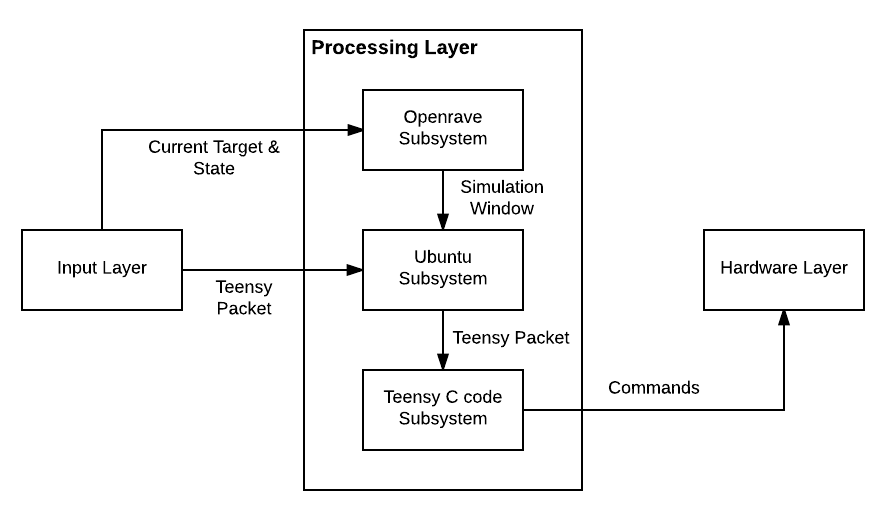
\includegraphics[width=0.60\textwidth]{images/processing}
 \caption{Processing Layer subsystem diagram}
\end{figure}

\subsection{OpenRave Subsystem}
The OpenRave Subsystem will simulate the movement of the robot arm and calculate the kinematics to find the optimal path to send to the arm.

\subsubsection{Assumptions}
The OpenRave subsystem will be able to simulate the arm accurately and be able to make accurate calculations

\subsubsection{Responsibilities}
This subsystem is responsible for using the simulation as well as calculate the kinematics needed to find the most accurate path for the robot arm to take, and is also responsible for communicating this data to the system.

\subsubsection{OpenRave Interfaces}

\begin {table}[H]
\caption {Subsystem interfaces} 
\begin{center}
    \begin{tabular}{ | p{1cm} | p{6cm} | p{3cm} | p{3cm} |}
    \hline
    ID & Description & Inputs & Outputs \\ \hline
    \#1 & Data in the form of a packet & \pbox{3cm}{Current target and state} & \pbox{3cm}{None}  \\ \hline
    \#2 & Simulation Window data & \pbox{3cm}{N/A} & \pbox{3cm}{Simulation window}  \\ \hline
    \end{tabular}
\end{center}
\end{table}

\subsection{Ubuntu Subsystem}
The Ubuntu Subsystem is what hosts the GUI and OpenRave simulation and sends data to the Teensy board.

\subsubsection{Assumptions}
The Ubuntu subsystem will be able to adequately host the application and be able to communicate with the Teensy board

\subsubsection{Responsibilities}
This subsystem is responsible for hosting the application and simulation while communicating with the Teensy board through a USB connection.

\subsubsection{Subsystem Interfaces}

\begin {table}[H]
\caption {Ubuntu interfaces} 
\begin{center}
    \begin{tabular}{ | p{1cm} | p{6cm} | p{3cm} | p{3cm} |}
    \hline
    ID & Description & Inputs & Outputs \\ \hline
    \#1 & Data in the form of a packet & \pbox{3cm}{Teensy Packet (from the GUI)} & \pbox{3cm}{Teensy Packet (to the Teensy)}  \\ \hline
    \#2 & Simulation Window data & \pbox{3cm}{N/A} & \pbox{3cm}{Simulation window display}  \\ \hline
    \end{tabular}
\end{center}
\end{table}

\subsection{Teensy C-Code Subsystem}
The Teensy C Code subsystem has the code to send commands to the hardware.

\subsubsection{Assumptions}
The Teensy C Code subsystem will be coded to send commands to operate the hardware accurately.

\subsubsection{Responsibilities}
This subsystem is responsible for receiving the packet data and using it to communicate with and send commands to the hardware subsystems to operate them. 

\subsubsection{Subsystem Interfaces}

\begin {table}[H]
\caption {Teensy interfaces} 
\begin{center}
    \begin{tabular}{ | p{1cm} | p{6cm} | p{3cm} | p{3cm} |}
    \hline
    ID & Description & Inputs & Outputs \\ \hline
    \#1 & Data in the form of a packet & \pbox{3cm}{Teensy packet data} & \pbox{3cm}{None}  \\ \hline
    \#2 & Command data & \pbox{3cm}{N/A} & \pbox{3cm}{Commands}  \\ \hline
    \end{tabular}
\end{center}
\end{table}
\newpage
\section{Hardware Layer Subsystems}


\begin{figure}[h!]
	\centering
 	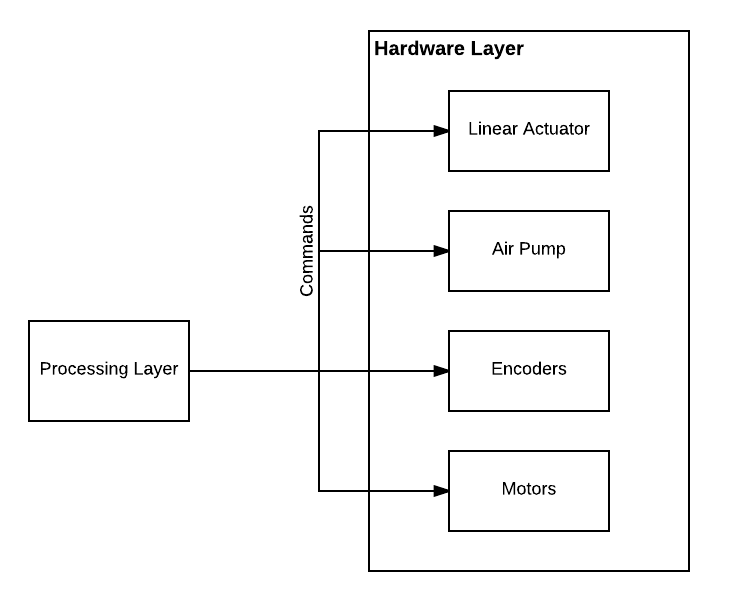
\includegraphics[width=0.60\textwidth]{images/hardware}
 \caption{Hardware Layer subsystem diagram}
\end{figure}

\subsection{Linear Actuator Subsystem}
The linear actuator is what moves the end effector down and up in order to grip an object

\subsubsection{Assumptions}
The subsystem will be able to receive commands in order to know when to operate its movement

\subsubsection{Responsibilities}
This subsystem is responsible for receiving its commands and making its movements when it should in a timely manner.

\subsubsection{Subsystem Interfaces}


\begin {table}[H]
\caption {Linear Actuator interfaces} 
\begin{center}
    \begin{tabular}{ | p{1cm} | p{6cm} | p{3cm} | p{3cm} |}
    \hline
    ID & Description & Inputs & Outputs \\ \hline
    \#1 & Command Data from Teensy & \pbox{3cm}{Commands} & \pbox{3cm}{Actuator movement}  \\ \hline

    \end{tabular}
\end{center}
\end{table}

\subsection{Motor Step Movement Subsystem}
The Stepper Motors are what moves the joints of the robot arm.

\subsubsection{Assumptions}
The subsystem will be able to receive commands in order to know when to operate its movement

\subsubsection{Responsibilities}
This subsystem is responsible for receiving its commands and making its movements when it should in a timely manner.

\subsubsection{Subsystem Interfaces}


\begin {table}[H]
\caption {Motor interfaces} 
\begin{center}
    \begin{tabular}{ | p{1cm} | p{6cm} | p{3cm} | p{3cm} |}
    \hline
    ID & Description & Inputs & Outputs \\ \hline
    \#1 & Command Data from Teensy & \pbox{3cm}{Commands} & \pbox{3cm}{Motor movement}  \\ \hline

    \end{tabular}
\end{center}
\end{table}

\subsection{Encoder Position Subsystem}
The Encoder subsystem should be able to take the angle of the arm joints and communicate the angle positions in order to provide motion control.

\subsubsection{Assumptions}
The subsystem will be able to receive commands in order to know when to operate its control

\subsubsection{Responsibilities}
This subsystem is responsible for receiving its commands and controling the movement accurately.

\subsubsection{Subsystem Interfaces}


\begin {table}[H]
\caption {Encoder interfaces} 
\begin{center}
    \begin{tabular}{ | p{1cm} | p{6cm} | p{3cm} | p{3cm} |}
    \hline
    ID & Description & Inputs & Outputs \\ \hline
    \#1 & Command Data from Teensy & \pbox{3cm}{Commands} & \pbox{3cm}{Encoder Position}  \\ \hline

    \end{tabular}
\end{center}
\end{table}

\subsection{Air Pump Subsystem}
This subsystem receives commands to operate the vacuum air pump which manipulates the gripper and allows the gripper to hold onto objects.

\subsubsection{Assumptions}
The subsystem will be able to receive commands in order to know when to operate vacuum.

\subsubsection{Responsibilities}
This subsystem is responsible for receiving its commands and operating when it should in a timely manner.

\subsubsection{Subsystem Interfaces}


\begin {table}[H]
\caption {Air Pump interfaces} 
\begin{center}
    \begin{tabular}{ | p{1cm} | p{6cm} | p{3cm} | p{3cm} |}
    \hline
    ID & Description & Inputs & Outputs \\ \hline
    \#1 & Command Data from Teensy & \pbox{3cm}{Commands} & \pbox{3cm}{Air pump operation}  \\ \hline

    \end{tabular}
\end{center}
\end{table}
\newpage

%%% References
\bibliographystyle{plain}
\bibliographystyle{reference/IEEEtran_custom}
\bibliography{reference/refs}{}

\end{document}